% This LaTeX file contains your written lab questions.  You may answer these
% questions just by inserting your answer into this document.  You are not
% *required* to do your homework in LaTeX, but it's quite likely to be easier
% than e.g. the equation editor in OpenOffice Writer or Microsoft Word.
\documentclass{article}

\usepackage{amsmath}
\usepackage{amssymb}
\usepackage{algpseudocode}
\usepackage{algorithmicx}
\usepackage{tikz}

\usetikzlibrary{positioning}

\begin{document}

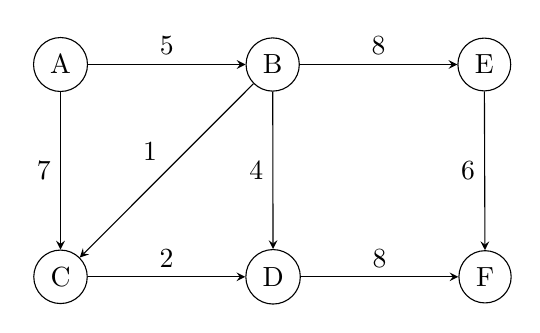
\begin{tikzpicture}[node distance=20mm and 20mm]
    \tikzstyle{vertex}=[circle,draw]
    \tikzstyle{edge}=[-stealth]
    
    \node[vertex] (A) {A};
    \node[vertex] (B) [right=of A] {B};
    \node[vertex] (C) [below=of A] {C};
    \node[vertex] (D) [right=of C] {D};
    \node[vertex] (E) [right=of B] {E};
    \node[vertex] (F) [right=of D] {F};
    
    \draw[edge] (A) to node[above] {5} (B);
    \draw[edge] (A) to node[left] {7} (C);
    \draw[edge] (B) to node[above left] {1} (C);
    \draw[edge] (B) to node[left] {4} (D);
    \draw[edge] (B) to node[above] {8} (E);
    \draw[edge] (C) to node[above] {2} (D);
    \draw[edge] (D) to node[above] {8} (F);
    \draw[edge] (E) to node[left] {6} (F);
\end{tikzpicture}

\vspace*{5mm}\par\textbf{Problem 1.} Perform a breadth-first search of the graph starting from vertex A.  Give the number of steps to reach \emph{every} other vertex.  Additionally, give the order in which the vertices are \emph{first} witnessed; that is, give the order in which they first enter the queue (and not necessarily the order in which they are explored).\par

\bigskip
The following represents the queue as DFS is preformed on the graph
\begin{enumerate}
    \item queue: B, C
    \item queue: C, E, D
    \item queue: E, D
    \item queue: D, F
    \item queue: F
\end{enumerate}

The number of steps to reach every other vertex is 5. The order in which each vertex is added to the queue is 
B, C, E, D, F. 

\vspace*{10mm}\par\textbf{Problem 2.} Use Dijkstra's algorithm on this graph starting from vertex A.  Give the cost of the least-cost path to \emph{every} other vertex.  Additionally, give the order in which the vertices are \emph{first} witnessed; that is, give the order in which they first enter the equeue (and not necessarily the order in which they are explored).\par

The following represents the piority queue as SSSP is preformed.

\begin{enumerate}
    \item queue: 5:B, 7:C 
    \item queue: 6:C, 7:C. 9:D, 13:E
    \item queue: 7:C. 8:D, 9:D, 13:E
    \item queue: 8:D, 9:D, 13:E
    \item queue: 9:D, 13:E. 16:F
    \item queue: 13:E. 16:F
    \item queue: 16:F, 19:F
    \item queue: 19:F
    \item queue: empty
\end{enumerate}

The least cost to reach each node is the following: B:5, C:6, D:8, E:13, F:16

The order in which the vertex are first witnessed is B, C, D, E, F.

\vspace*{10mm}\par\textbf{Problem 3.} Give two valid topological sorts of this graph.\par



\begin{center}
    \begin{tabular}{||c c||} 
     \hline
     Sort 1 & Sort 2\\ [0.5ex] 
     \hline\hline
     A & A  \\ 
     \hline
     B & B \\
     \hline
     E & C \\
     \hline
     C & D  \\
     \hline
     D & E \\  
     \hline
     F & F \\ [1ex] 
     \hline
    \end{tabular}
\end{center}


\end{document}
